results

general outline:

\begin{itemize}
\item full core model
	\begin{itemize}
	\item radial banding on outer edge due to pebble location
	\item to a lesser degree, axial banding on top/bottom
	\item while not symmetrical, 'hot spots' are fairly rare, and a general gradient in the fission rate (orange) can be seen.
	\item noticeable hotspots seem to be at the very top/bottom, in the middle, and at the edges in the radial image.  Of course, this isn't seen in the axial mesh, because the edges of the axial mesh are only integrating over a small amount of material, while in the radial mesh, all parts integrate over the entire height of the reactor.
	\item ***One point of interest (discuss in meeting?)*** is that theoretically, the centerline of the axial mesh should all be integrating over the same amount of material - a thickness corresponding to the diameter of the reactor, 165 inches, which is also the height.  However, the hotspots I see at the top and bottom in the center aren't carried through the centerline.  If the hotspots in the top and bottom of the axial mesh were simply because it integrated over more material, shouldn't the entire centerline be brighter?
	\item I do notice a *very slight* trend to the right side of the axial mesh, at least toward the bottom
	\item since the radial mesh is integrating over the same volume throughout, I expected it to show the sort of trend in fission rate I would expect from a cylindrical reactor - more intense at the center, tapering toward the edge.  Certainly, the reflector (blue) is doing that with scatters.  But why is the center so dark compared to the outside?  is the banding that intense?
		\begin{itemize}
		\item had a thought: the meshes integrate over space, right.  It so happens that the bands here are where pebbles are perfectly lining up.  What if this intensity at the edges is a misrepresentation, a limitation of how the mesh is made?  If integrating over space, and all the the space in that section are pebbles - ie, fuel, remember they are homogenized - then the effect is that the integrated space is more concentrated.  As you go towards the center, and pebble location becomes random, the same 'section' integrated in isn't just fuel pebbles anymore, there could also be coolant.  It's 'watering down' that section.  If you look at the axial mesh, at the left and right edges you can see exactly what one pebble looks like, and it's rather dark
		\end{itemize}
	\end{itemize}
	
\item sensitivity and symmetry
	\begin{itemize}
	\item no noticeable change in the k-eff between runs, for either switching pebble comps or going to a 1/6th core
	\item banding behavior highlights a potential issue in using symmetry, but for 1/6th did not significantly change the overall trends in the mesh figures
	\item notably, I did compare the meshes, and for the radial symmetry at least, is is quite literally just taking the corresponding portion of the full core control and reflecting it around (i expected a little bit of a difference at least)
	\end{itemize}
\item flux
	\begin{itemize}
	\item radial and axial fluxes, two group
	\item 2 group flux in a fresh and 6pass pebble
	\end{itemize}
	
\end{itemize}
\section{Full-Core Control Model}

\begin{figure}[H]
\centering
%
\begin{subfigure}{0.4\textwidth}
  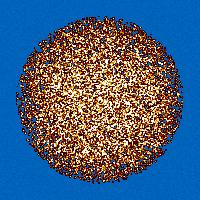
\includegraphics[width=0.95\linewidth]{figures/burn-20-bstep0}
  \caption{Fresh}
  \label{fig:bstep0}
\end{subfigure}%
%
\begin{subfigure}{0.4\textwidth}
  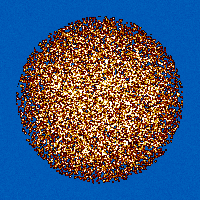
\includegraphics[width=0.95\linewidth]{figures/burn-20-bstep1}
  \caption{One Pass}
  \label{fig:bstep1}
\end{subfigure}%

\caption{Mesh Figures For Single Pebble Burnup}
\end{figure}

\begin{figure}[H]\ContinuedFloat
\centering

\begin{subfigure}{0.4\textwidth}
  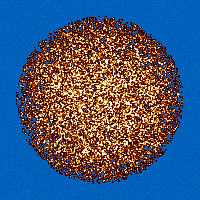
\includegraphics[width=0.95\linewidth]{figures/burn-20-bstep2}
  \caption{Two Passes}
  \label{fig:bstep2}
\end{subfigure}%
%
\begin{subfigure}{0.4\textwidth}
  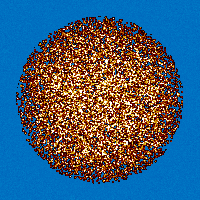
\includegraphics[width=0.95\linewidth]{figures/burn-20-bstep3}
  \caption{Three Passes}
  \label{fig:bstep3}
\end{subfigure}%

\begin{subfigure}{0.4\textwidth}
  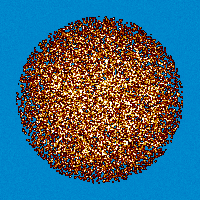
\includegraphics[width=0.95\linewidth]{figures/burn-20-bstep4}
  \caption{Four Passes}
  \label{fig:bstep4}
\end{subfigure}%
%
\begin{subfigure}{0.4\textwidth}
  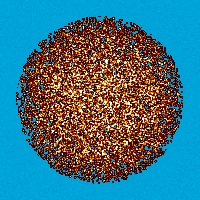
\includegraphics[width=0.95\linewidth]{figures/burn-20-bstep5}
  \caption{Five Passes}
  \label{fig:bstep5}
\end{subfigure}%

\begin{subfigure}{0.4\textwidth}
  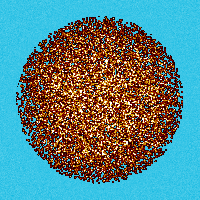
\includegraphics[width=0.95\linewidth]{figures/burn-20-bstep6}
  \caption{Six Passes}
  \label{fig:bstep6}
\end{subfigure}%
%
\caption{Mesh Figures For Single Pebble Burnup(cont.)}
\label{fig:burn-meshes}
\end{figure}
\begin{itemize}
\item meshes for each burnup used in single pebble
\item pebbles are not homogenized
\item each pass is six months
\item pebble is 3.0 cm across, with helium to fill out the cube it is inscribed in
\item each corresponds to a fuel composition in the full core
\item can see the outside (helium, material: blue) become paler over time (fewer scatters?)
\item can see the pebble (sphere, mat: non-homogenized pebble) become darker over time (fewer fissions?)
\end{itemize}

\begin{figure}[H]
\centering

\begin{subfigure}{0.45\textwidth}
  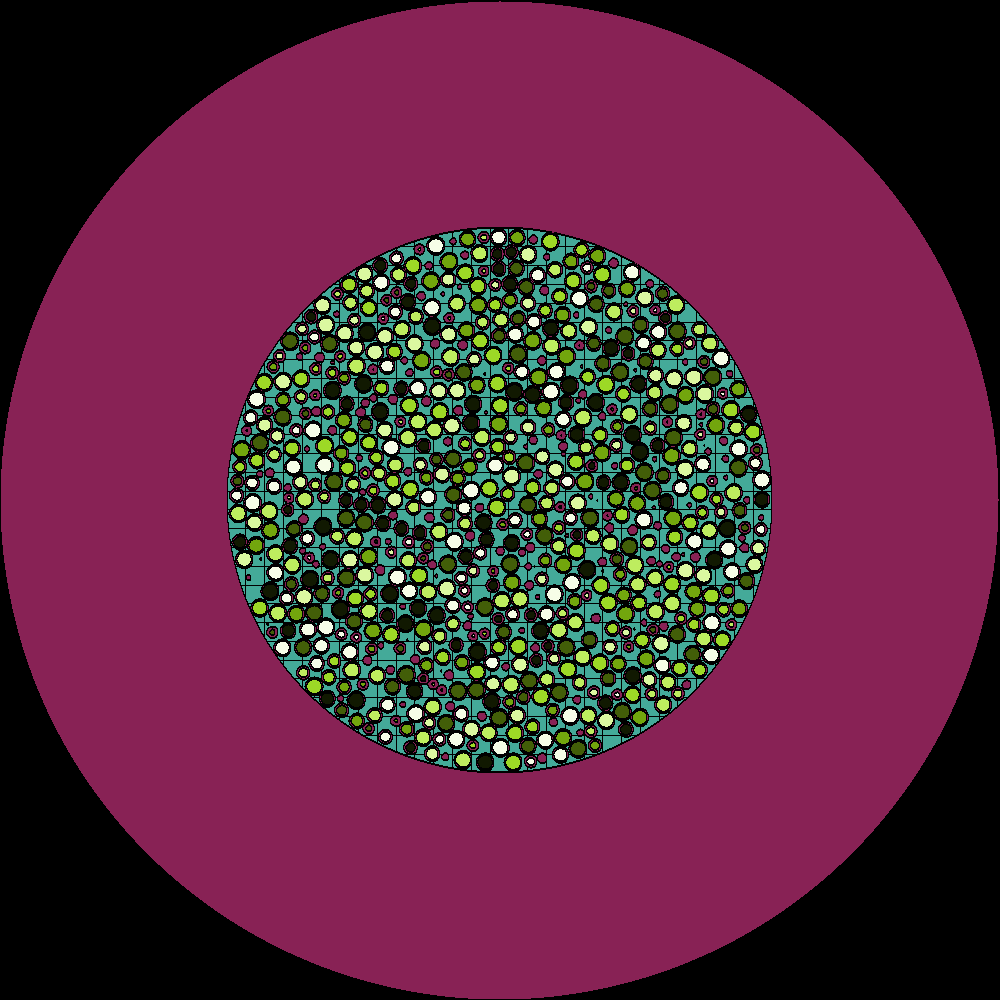
\includegraphics[width=0.95\linewidth]{figures/control/control-r}
  \caption{Radial Cross Section at y=0}
  \label{fig:controla}
\end{subfigure}%
%
\begin{subfigure}{0.45\textwidth}
  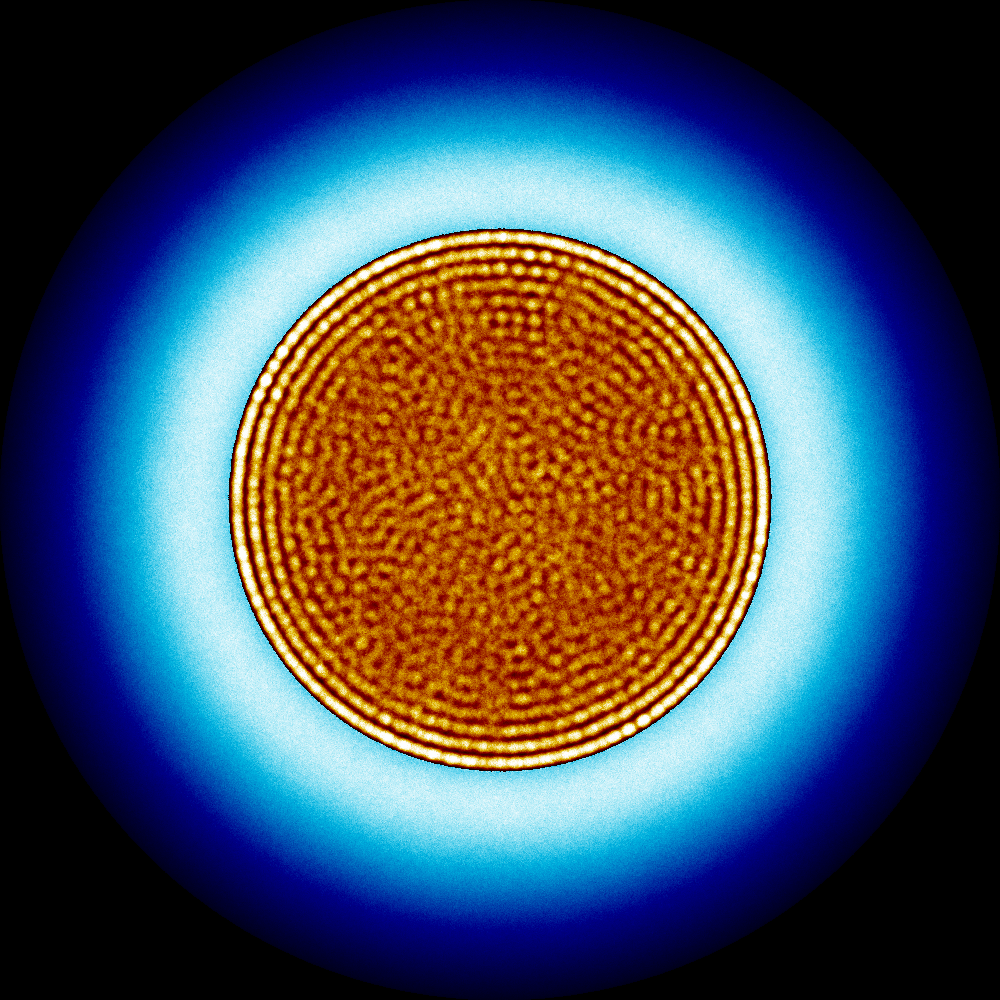
\includegraphics[width=0.95\linewidth]{figures/control/control-rm}
  \caption{Radial Mesh}
  \label{fig:controlb}
\end{subfigure}

\begin{subfigure}{0.45\textwidth}
  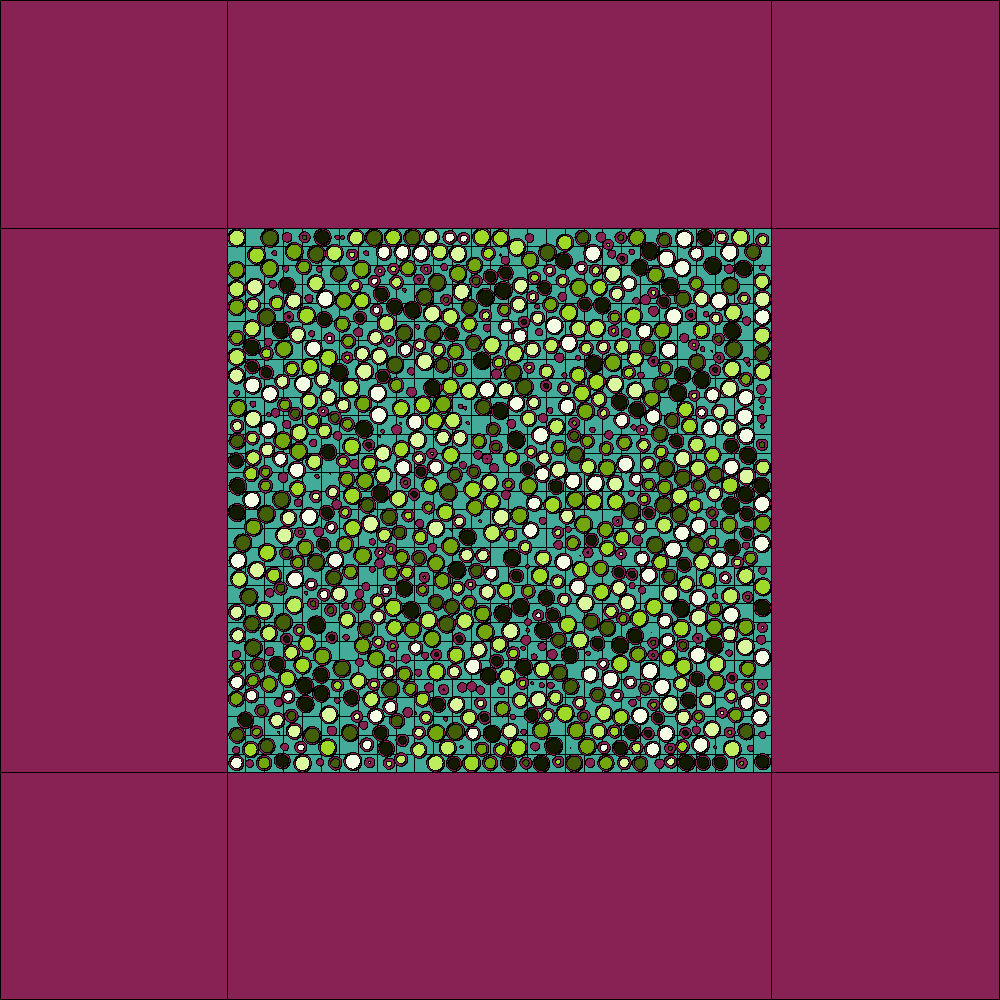
\includegraphics[width=0.95\linewidth]{figures/control/control-v}
  \caption{Axial Cross Section at z=0 }
  \label{fig:controlc}
\end{subfigure}
%
\begin{subfigure}{0.45\textwidth}
  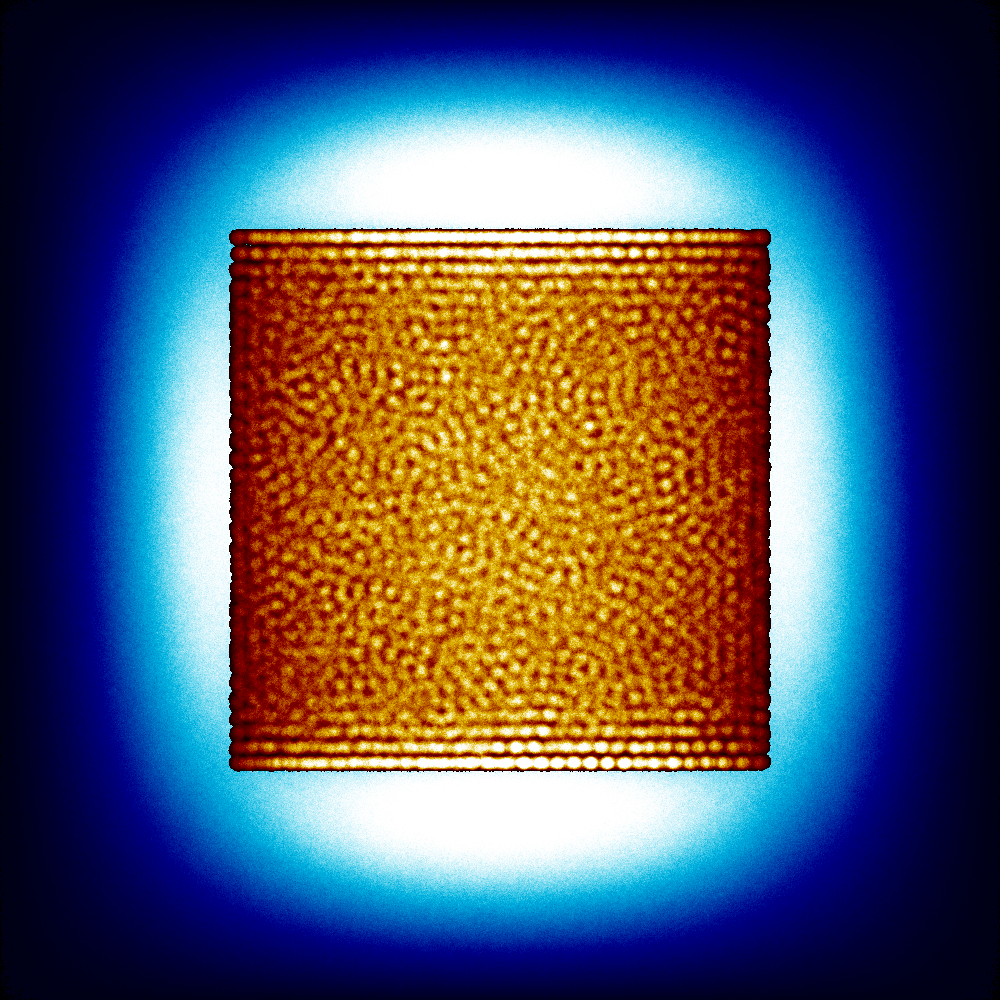
\includegraphics[width=0.95\linewidth]{figures/control/control-vm}
  \caption{Axial Mesh}
  \label{fig:controld}
\end{subfigure}
%
\begin{subfigure}{\textwidth}
\centering
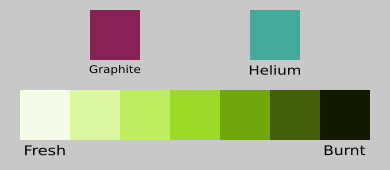
\includegraphics[width=0.6\linewidth]{figures/geom-legend}
\caption{Legend for \ref{fig:controla} and \ref{fig:controlc}}
\label{fig:geom-legend1}
\end{subfigure}

\caption{Geometry Cross Sections (left) and Thermal Flux(cold color map) and Fission Rate (hot color map) Meshes (right) for the Control Model of Sangamon20}
\label{fig:controlmain}
\end{figure}
\begin{itemize}
\item full core model
\item homogenized pebbles
\item no symmetry setting
\item rings due to pebbles naturally lining up along the outer edges due to the physical barrier of the graphite, then becoming more random towards the center
\item teal is helium
\item pink is graphite
\item pebbles green: lighter -> darker = fresh -> burnt
\item remember that the meshes are integrated to create the 2d representation, it is not the fission/scattering in that cross section alone
\end{itemize}

The burnup models of the single pebble inscribed in a cube of helium provide the middle-of-life compositions used in the Sangamon20 full-core models.  The exact compositions are provided in the appendix.  Overall, the behavior of the single-pebble burnup models over time are as expected.  As the pebble is more burned, the fission and scattering rates decrease in the fuel pebble and surrounding helium, respectively.  The presence of 'holes' in the mesh aren't unexpected - the packing fraction of TRISO particles in the pebbles is significantly lower than the packing fraction of pebbles in the reactor.

The homogenized pebbles in the full-core model are much more uniform throughout the pebble compared to the heterogeneous pebbles, as one might expect.  A more interesting feature is the presence of radial rings in the outer reactor core.  These rings are more clearly seen in the mesh, but as the geometry cross-section shows, this phenomenon is due to the physical layout of the pebbles.  Towards the outside, the pebbles have the walls of the reactor to line up against, and so their location is uniform.  As you approach the center, without a physical barrier, the pebbles are able to find more 'random' positions.  This phenomenon also makes sense when one considers the mechanics of the Serpent 2.0 growth and shake algorithm.  As discussed in the Methods chapter, the growth and shake factors are very small fractions of pebble radius.  The dispersal routine determines pebble locations iteratively, and once the initial center point is determined, moves and grows each pebble the minimum amount required to fit the routine's three criterion:  1) the particle is at its full size, 2) the particle doesn't overlap with any other particles,  and 3) the particle is fully contained in the boundaries of the container.  Naturally, then, any particle spawned relatively close to the outer bound would line up with it as the algorithm 'shakes' the particles.




\section{Sensitivity Tests}

\subsection{Effects of Symmetry Assumption}

\begin{figure}[h!]
\centering

\begin{subfigure}{0.45\textwidth}
  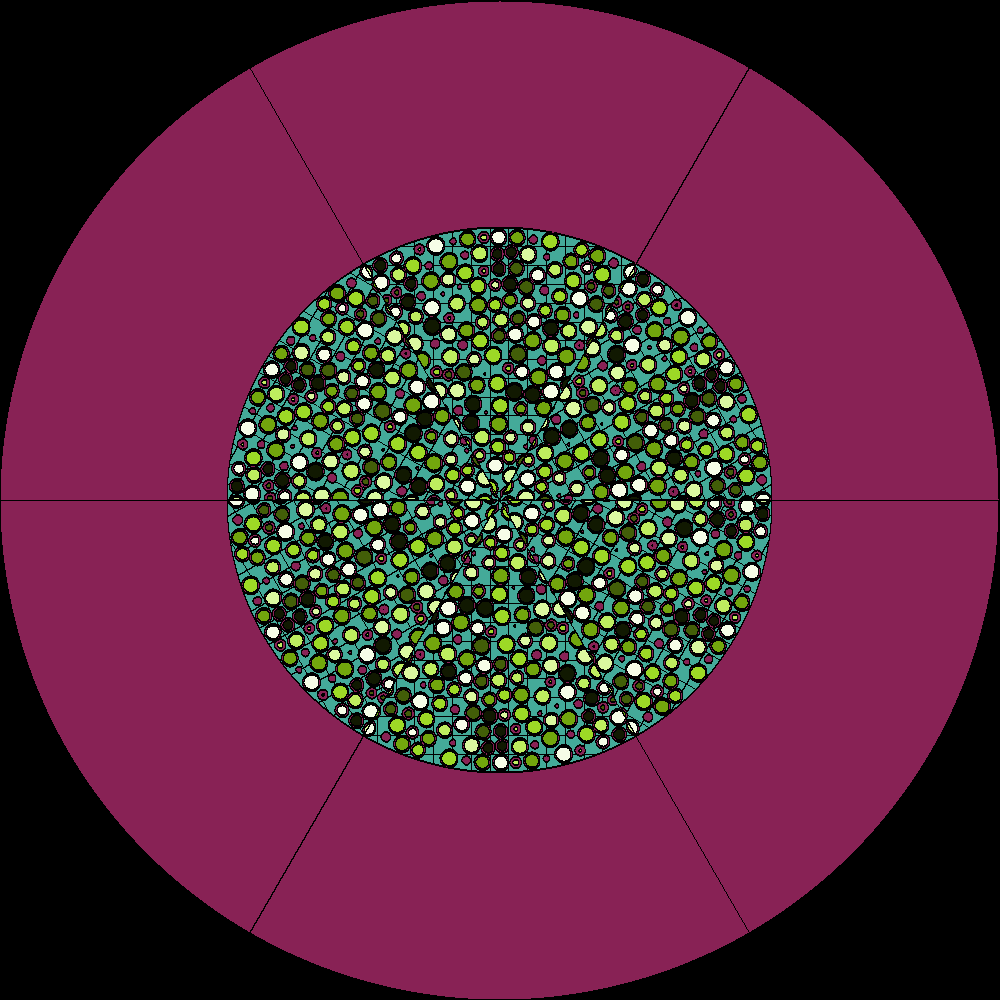
\includegraphics[width=0.95\linewidth]{figures/60-120/60-120-r}
  \caption{Radial Cross Section at y=0}
  \label{fig:bstep0}
\end{subfigure}%
%
\begin{subfigure}{0.45\textwidth}
  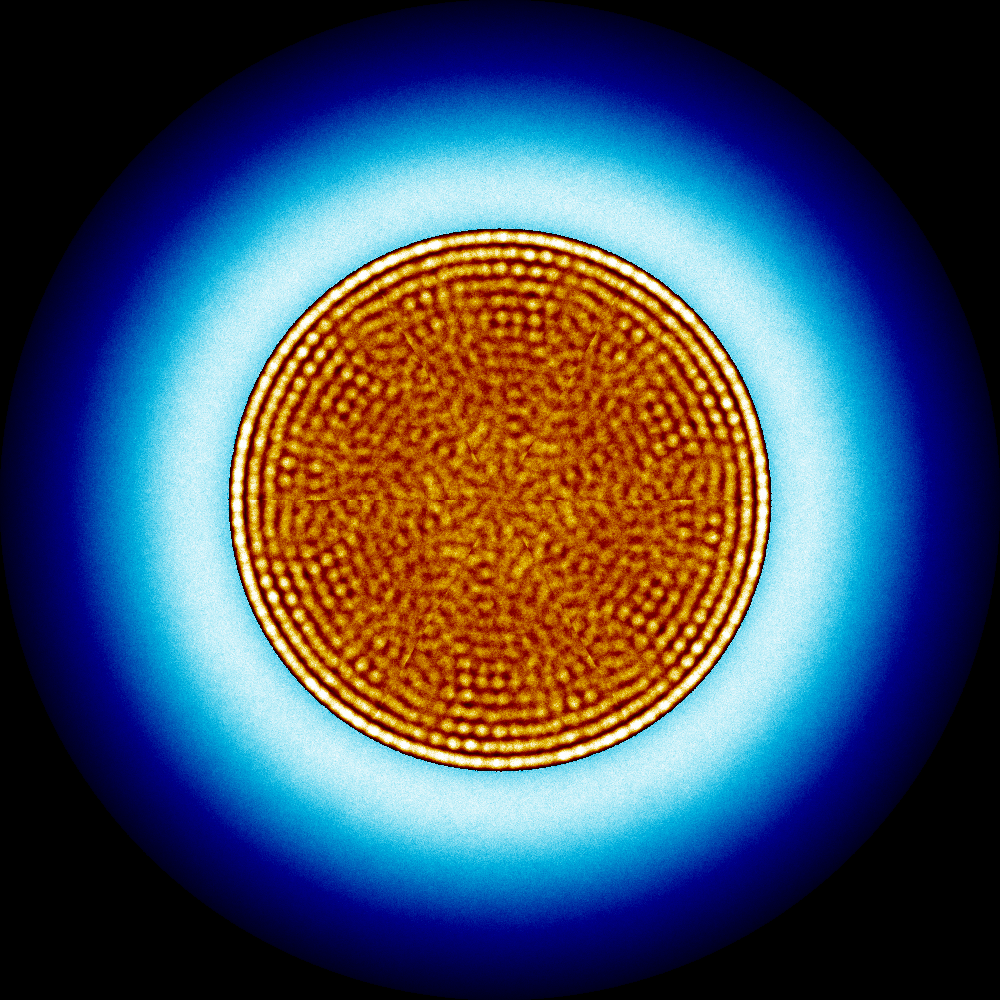
\includegraphics[width=0.95\linewidth]{figures/60-120/60-120-rm}
  \caption{Radial Mesh}
  \label{fig:bstep1}
\end{subfigure}

\begin{subfigure}{0.45\textwidth}
  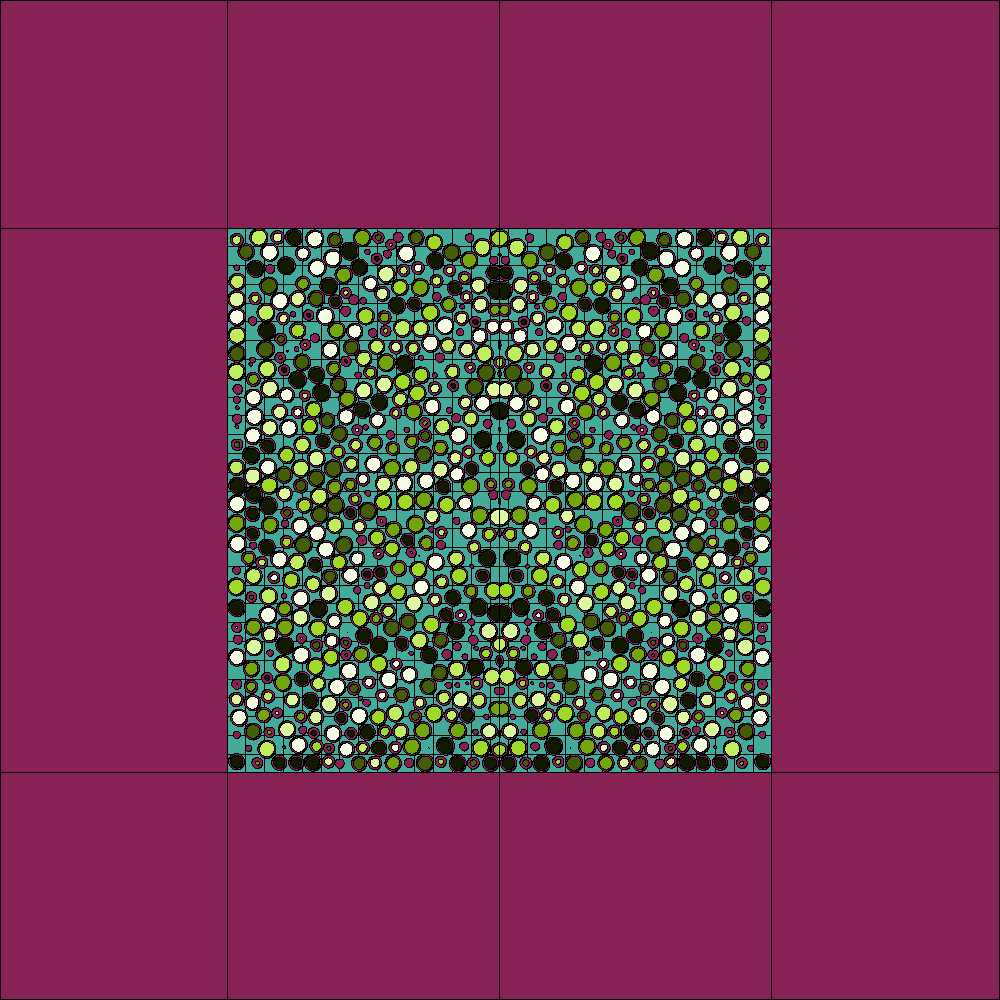
\includegraphics[width=0.95\linewidth]{figures/60-120/60-120-v}
  \caption{Axial Cross Section at z=0 }
  \label{fig:bstep1}
\end{subfigure}
%
\begin{subfigure}{0.45\textwidth}
  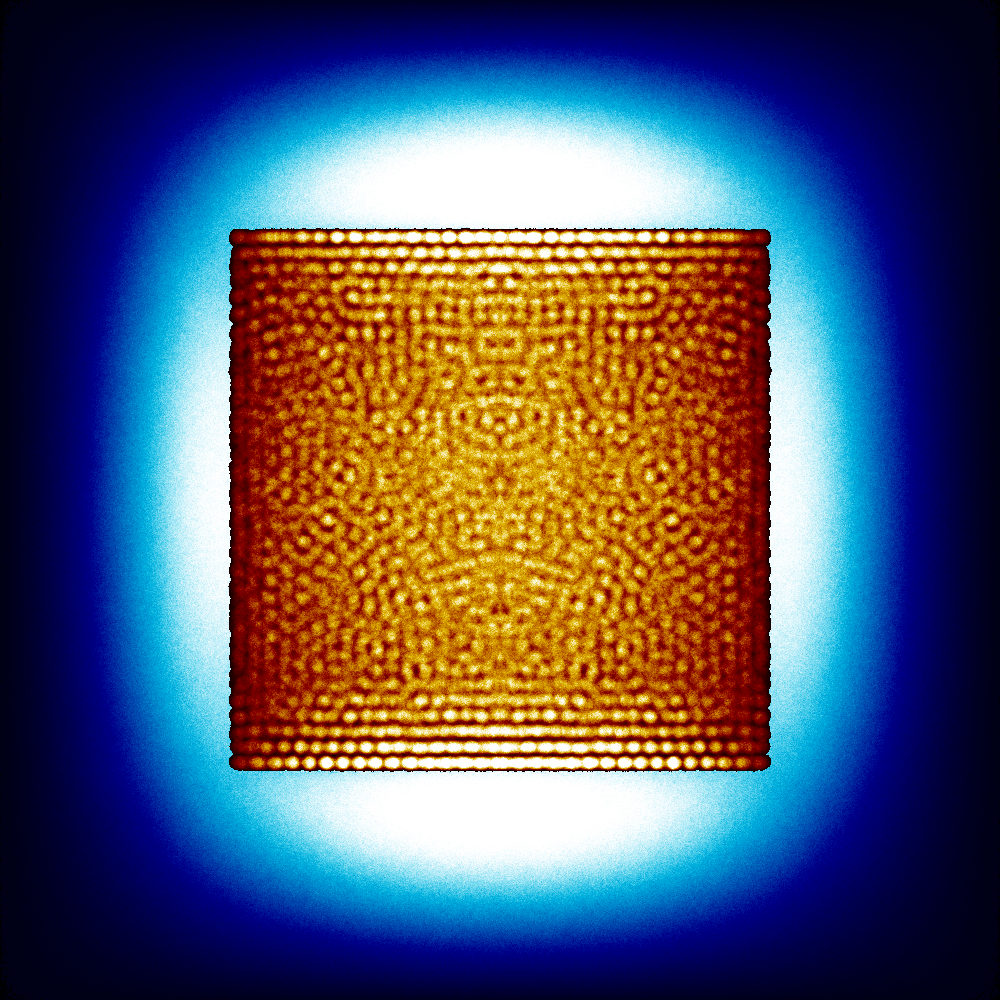
\includegraphics[width=0.95\linewidth]{figures/60-120/60-120-vm}
  \caption{Axial Mesh}
  \label{fig:bstep1}
\end{subfigure}
%
\caption{Sensitivity Analysis: $60^{\circ}$ - $120^{\circ}$}
\label{fig:60-120}
\end{figure}
\begin{itemize}
\item 1/6 core symmetry
\item uses the section of the core that is the 0-60 slice from the full core
\item periodic boundary condition between core 'slices' vacuum outside
\item the center cross section is slightly better to visualize the 'banding' or petal behavior of the pebbles, but the axial one is more representative of the banding patterns in the entire core.  Remember, the line the axial image cuts through to give us this image lays on the boundary of a slice (the line corresponding to the horizontal one in the radial geom cross section) this means that the patterns seen in the axial geom here are repeated at the borders of every slice.
\end{itemize}

\begin{figure}[H]
\centering

\begin{subfigure}{0.45\textwidth}
  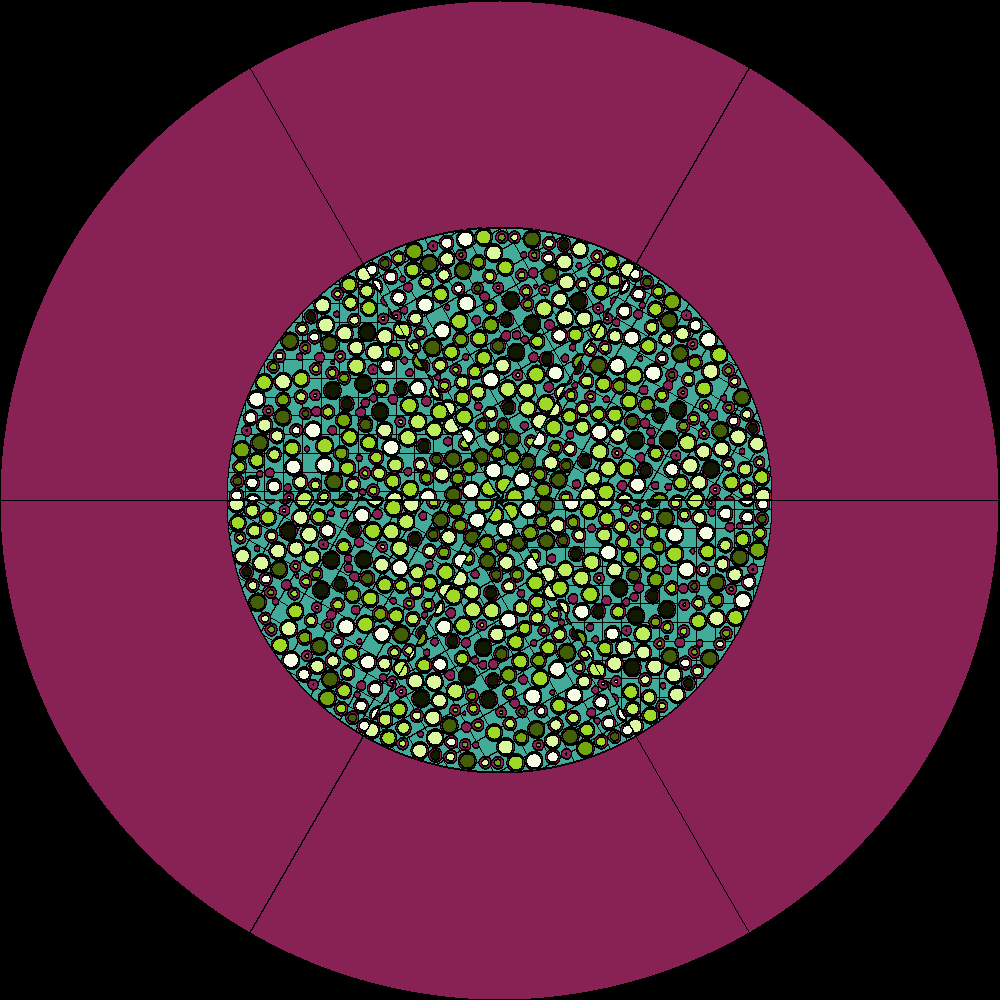
\includegraphics[width=0.95\linewidth]{figures/120-180/120-180-r}
  \caption{Radial Cross Section at y=0}
  \label{fig:120-180-r}
\end{subfigure}%
%
\begin{subfigure}{0.45\textwidth}
  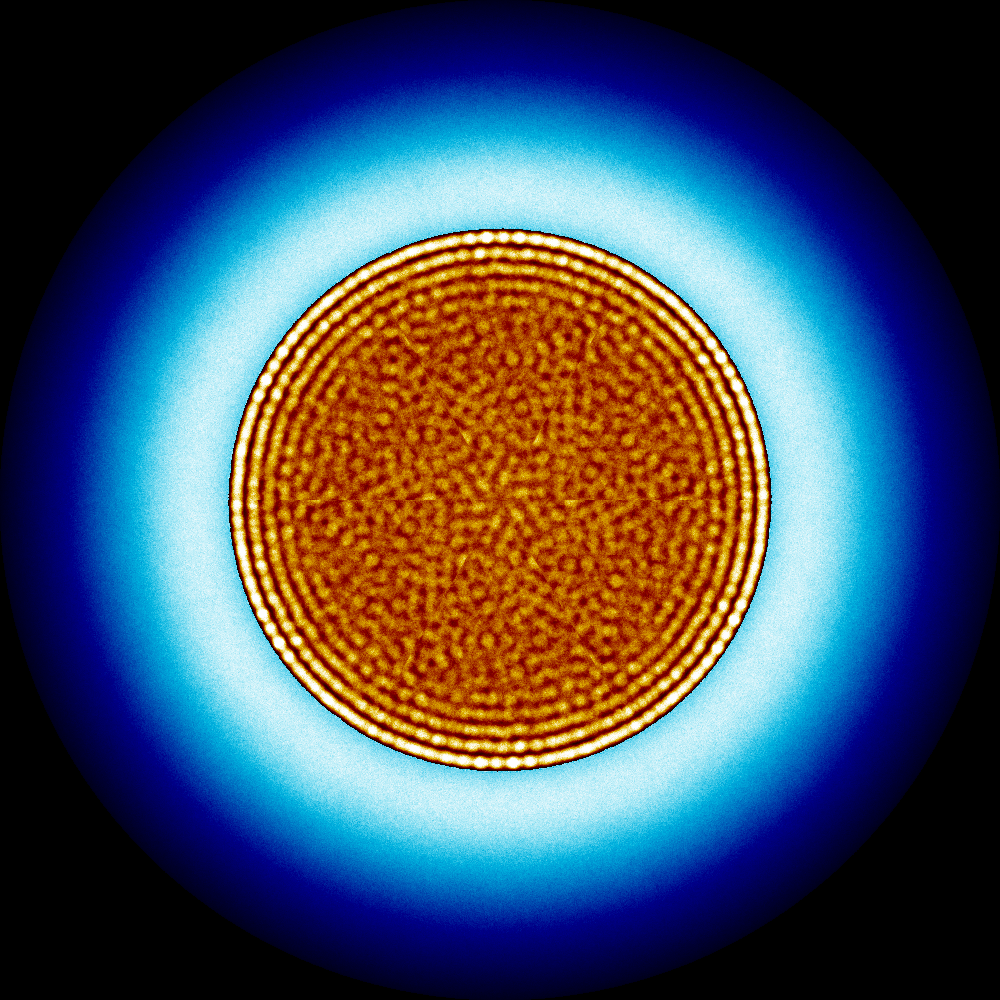
\includegraphics[width=0.95\linewidth]{figures/120-180/120-180-rm}
  \caption{Radial Mesh}
  \label{fig:120-180-rm}
\end{subfigure}

\begin{subfigure}{0.45\textwidth}
  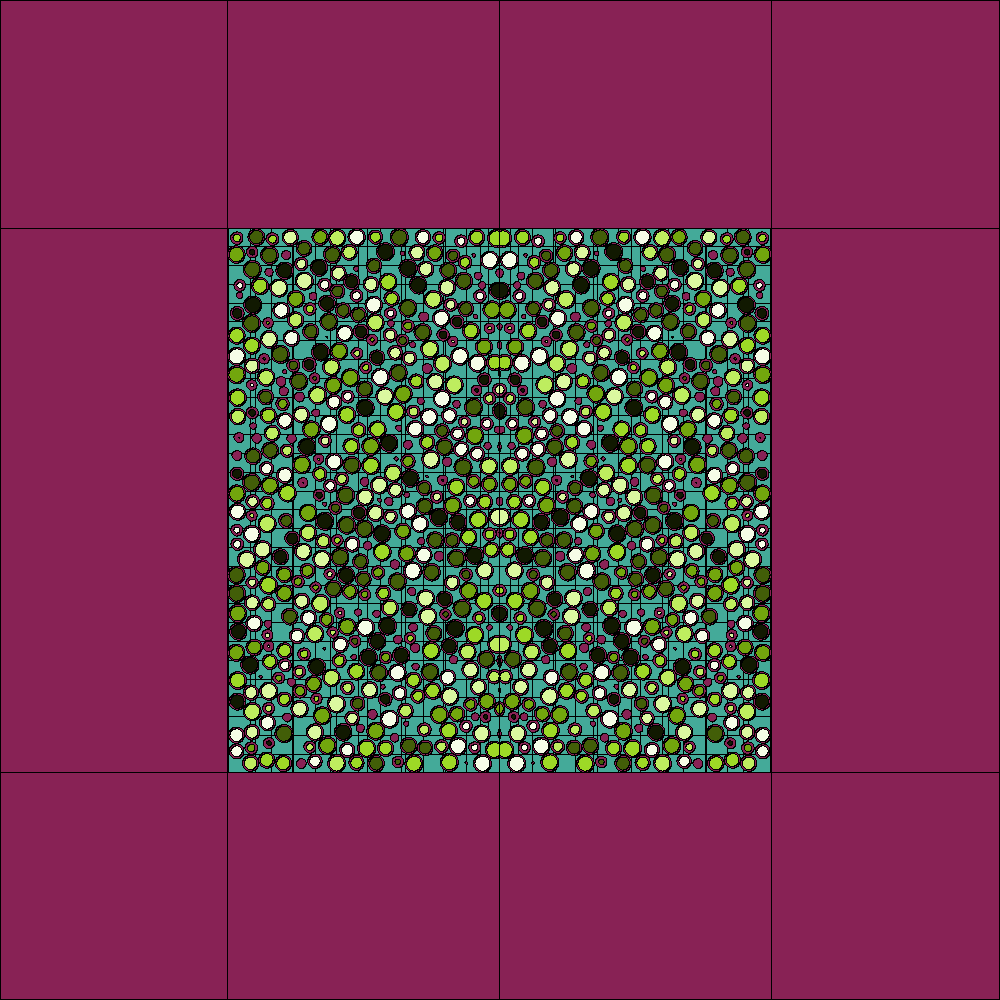
\includegraphics[width=0.95\linewidth]{figures/120-180/120-180-v}
  \caption{Axial Cross Section at z=0 }
  \label{fig:120-180-v}
\end{subfigure}
%
\begin{subfigure}{0.45\textwidth}
  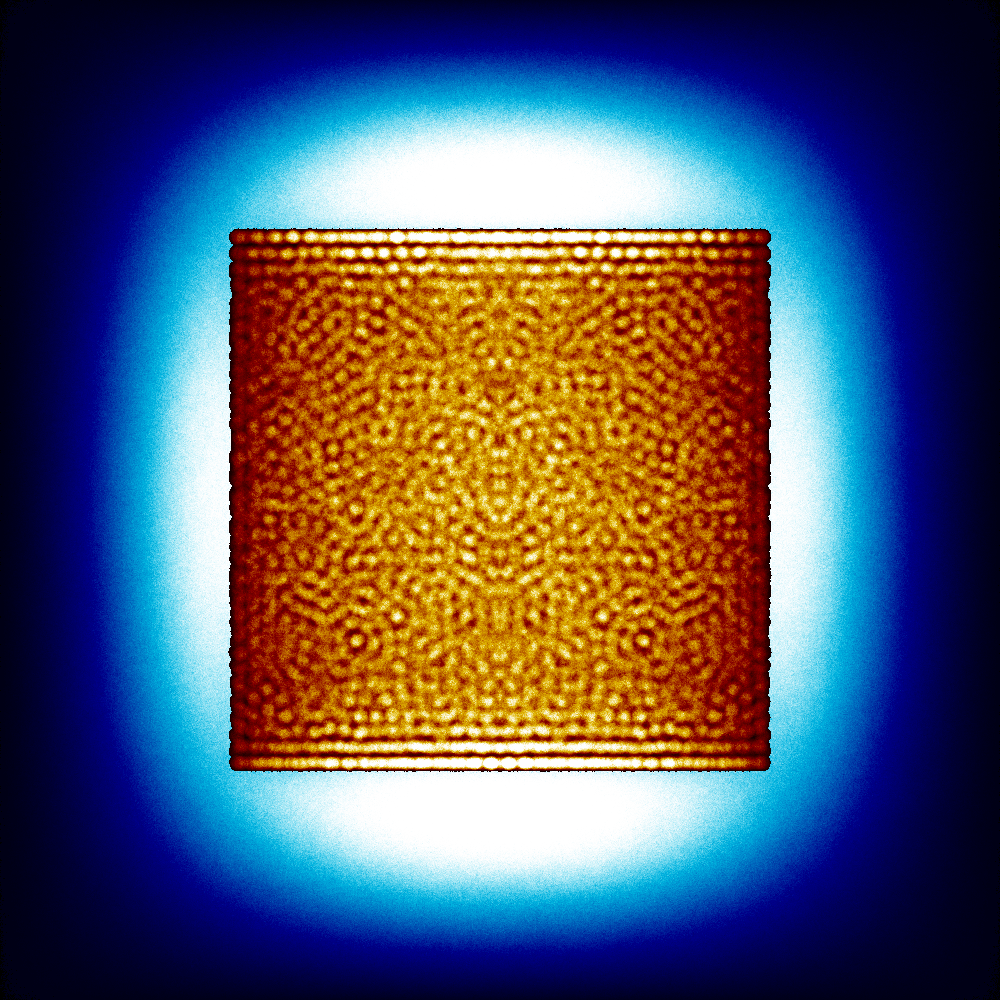
\includegraphics[width=0.95\linewidth]{figures/120-180/120-180-vm}
  \caption{Axial Mesh}
  \label{fig:120-180-vm}
\end{subfigure}
%
\caption{Sensitivity Analysis: $120^{\circ}$ - $180^{\circ}$}
\label{fig:120-180}
\end{figure}
\begin{itemize}
\item as above, but the 120-180 degree slice
\end{itemize}

\begin{figure}
\centering

\begin{subfigure}{0.45\textwidth}
  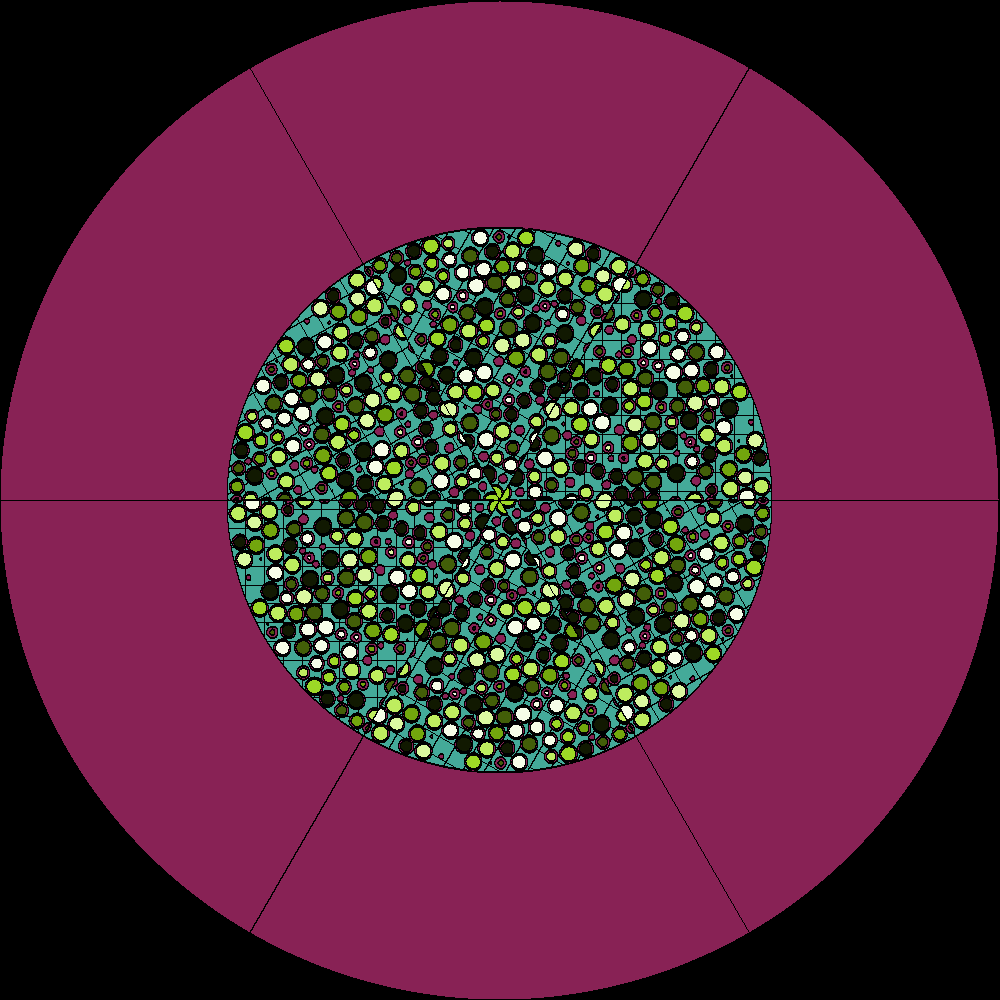
\includegraphics[width=0.95\linewidth]{figures/180-240/180-240-r}
  \caption{Radial Cross Section at y=0}
  \label{fig:bstep0}
\end{subfigure}%
%
\begin{subfigure}{0.45\textwidth}
  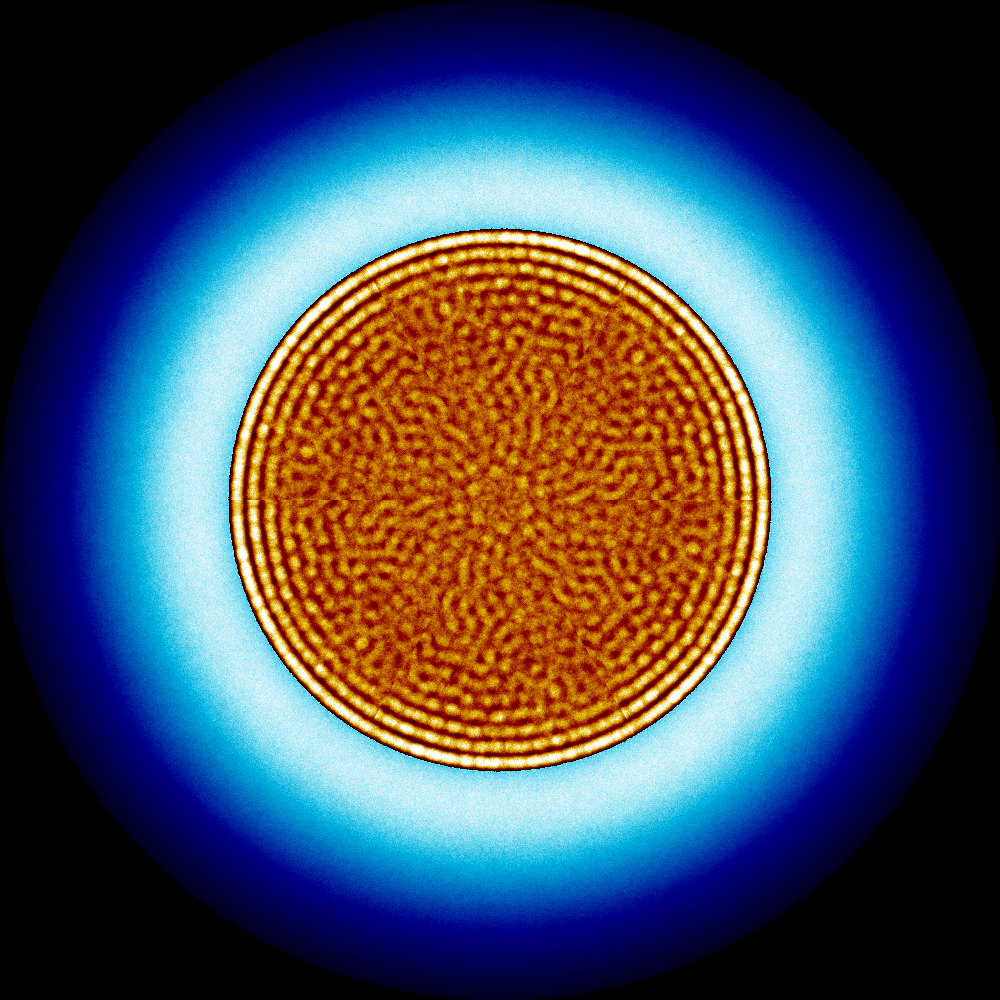
\includegraphics[width=0.95\linewidth]{figures/180-240/180-240-rm}
  \caption{Radial Mesh}
  \label{fig:bstep1}
\end{subfigure}

\begin{subfigure}{0.45\textwidth}
  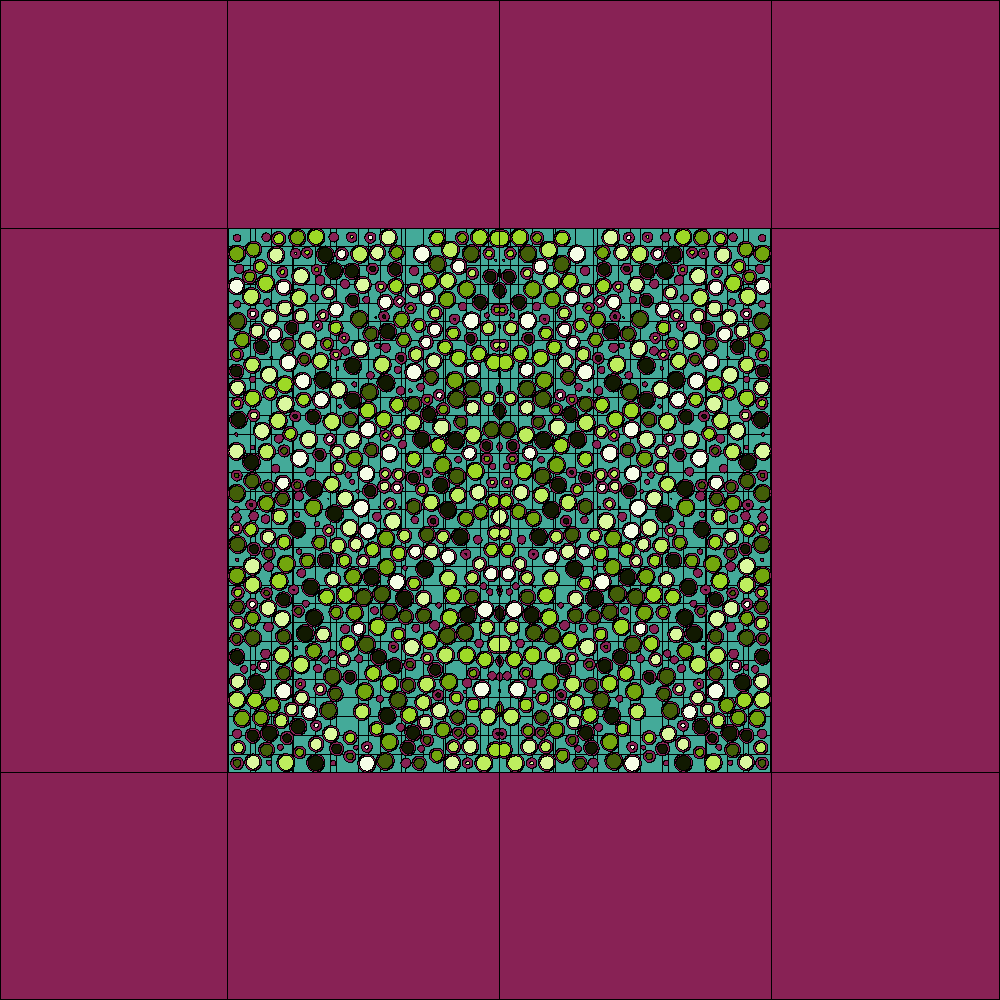
\includegraphics[width=0.95\linewidth]{figures/180-240/180-240-v}
  \caption{Axial Cross Section at z=0 }
  \label{fig:bstep1}
\end{subfigure}
%
\begin{subfigure}{0.45\textwidth}
  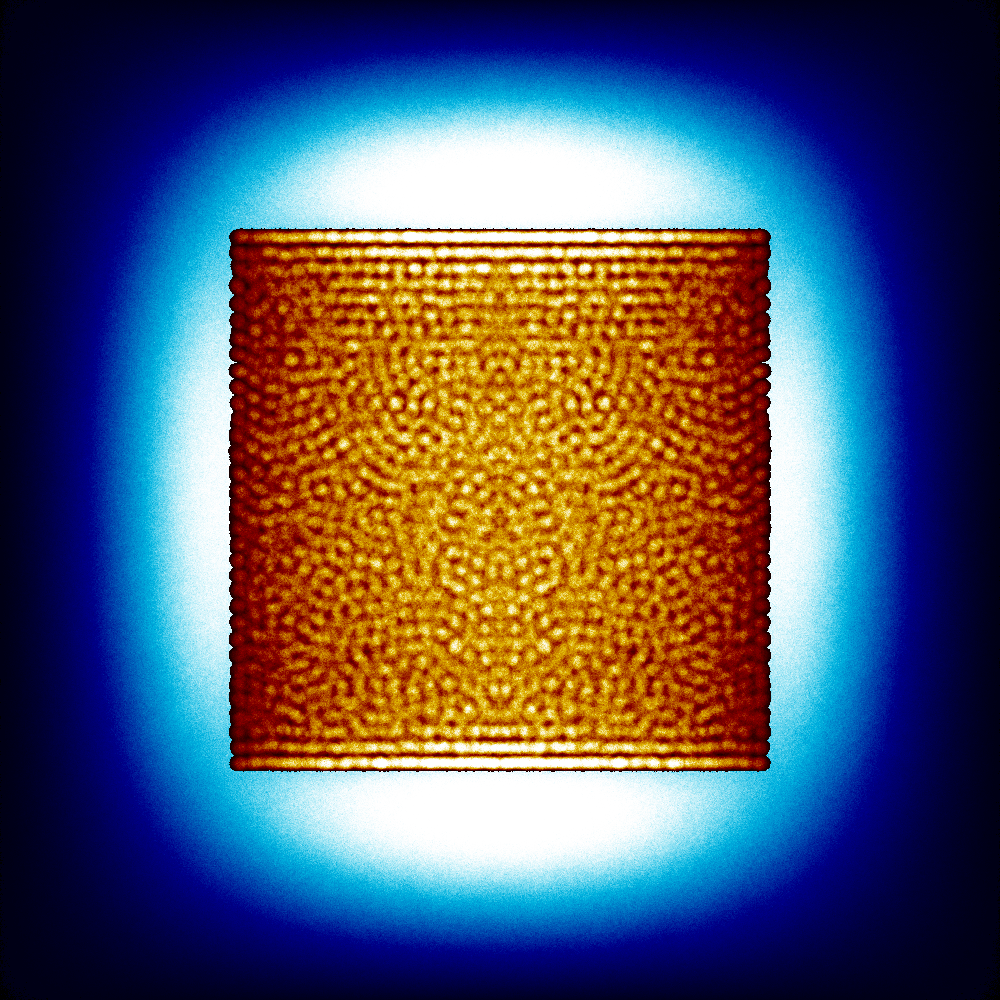
\includegraphics[width=0.95\linewidth]{figures/180-240/180-240-vm}
  \caption{Axial Mesh}
  \label{fig:bstep1}
\end{subfigure}
%
\caption{Sensitivity Analysis: $180^{\circ}$ - $240^{\circ}$}
\label{fig:180-240}
\end{figure}
\begin{itemize}
\item as above, but the 180-140 degree slice
\end{itemize}

\begin{figure}
\centering

\begin{subfigure}{0.45\textwidth}
  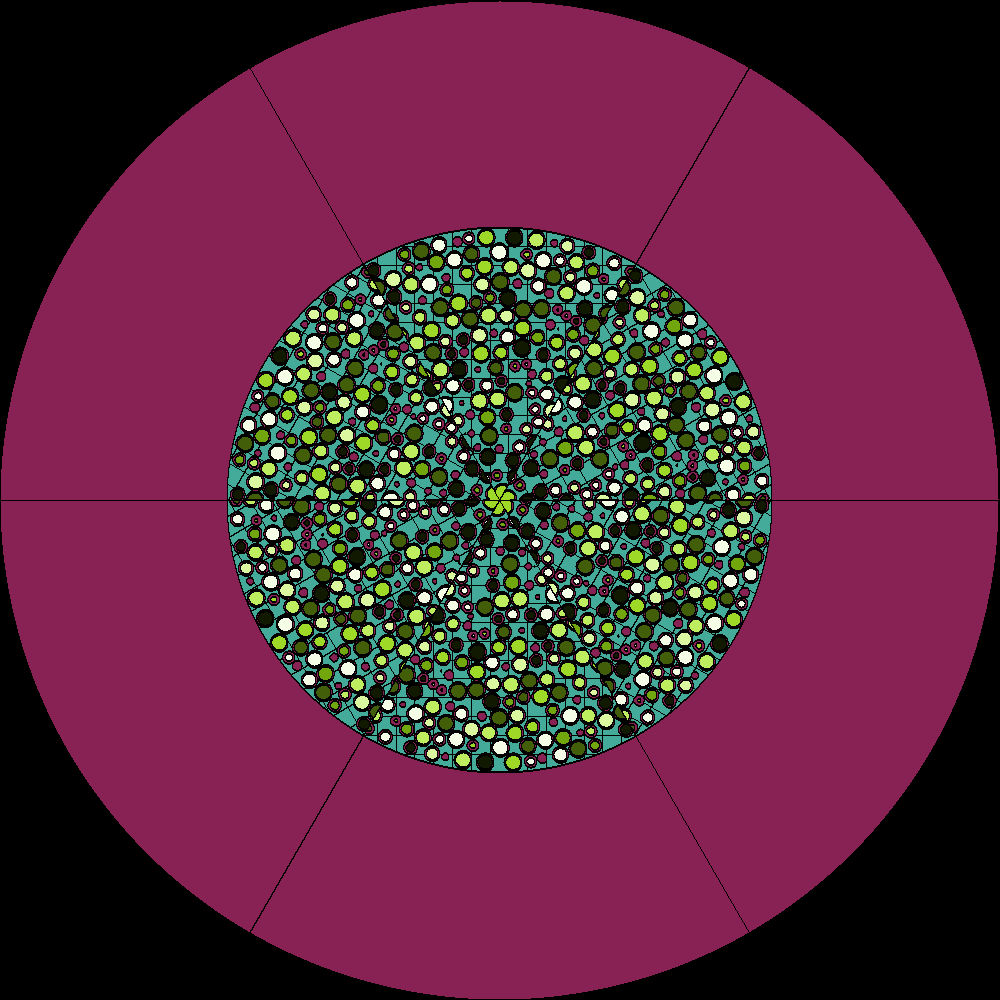
\includegraphics[width=0.95\linewidth]{figures/240-300/240-300-r}
  \caption{Radial Cross Section at y=0}
  \label{fig:bstep0}
\end{subfigure}%
%
\begin{subfigure}{0.45\textwidth}
  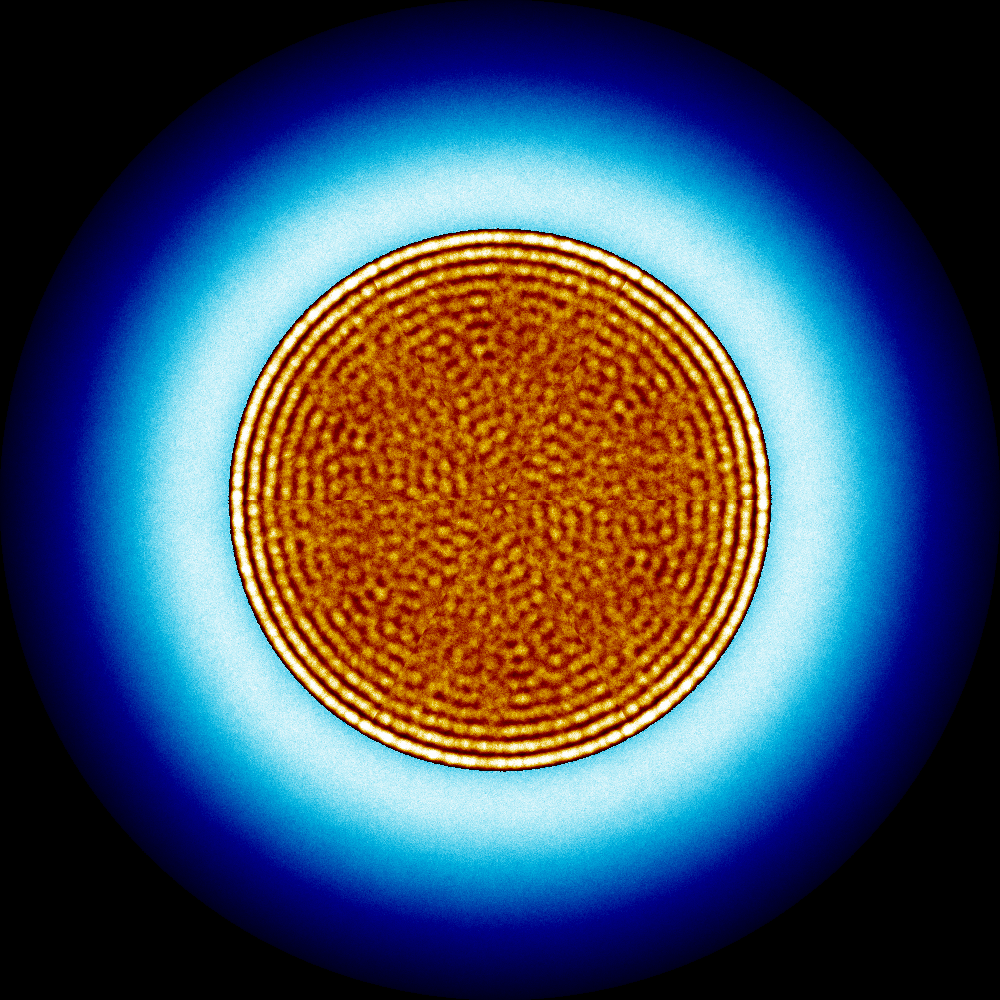
\includegraphics[width=0.95\linewidth]{figures/240-300/240-300-rm}
  \caption{Radial Mesh}
  \label{fig:bstep1}
\end{subfigure}

\begin{subfigure}{0.45\textwidth}
  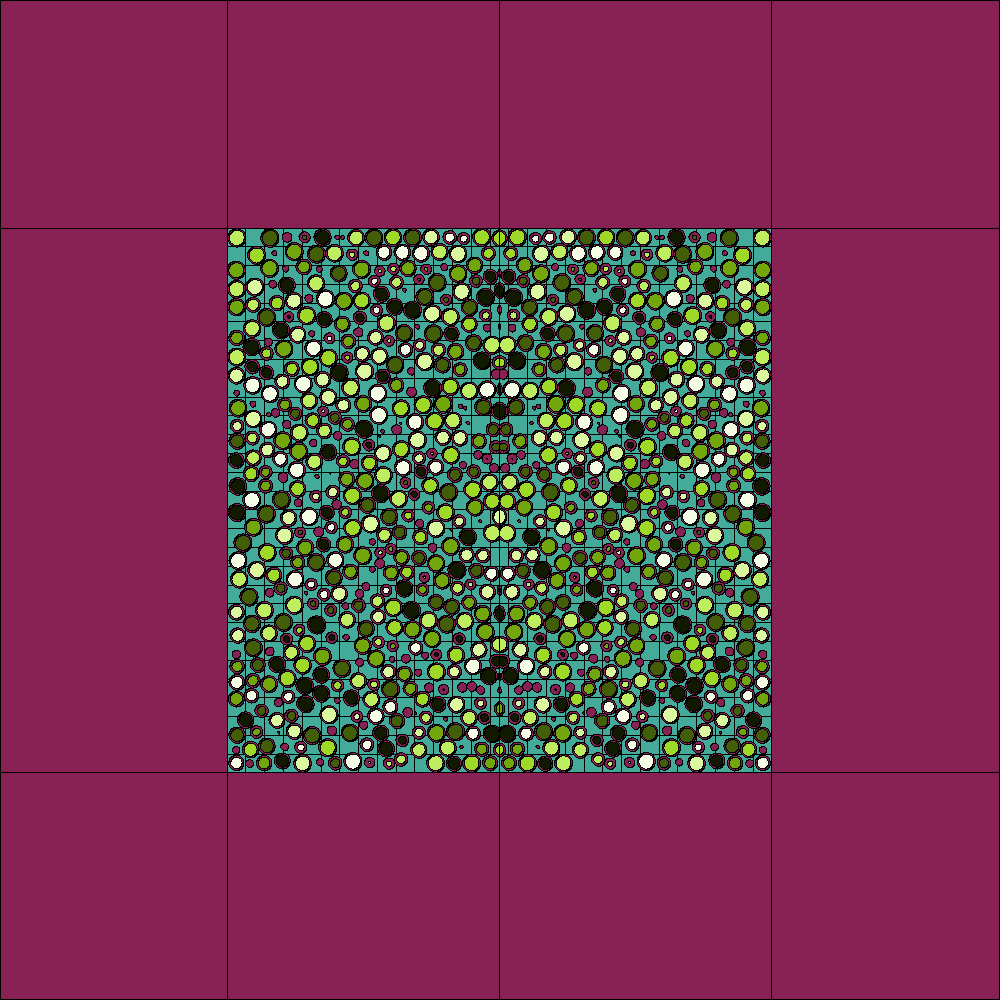
\includegraphics[width=0.95\linewidth]{figures/240-300/240-300-v}
  \caption{Axial Cross Section at z=0 }
  \label{fig:bstep1}
\end{subfigure}
%
\begin{subfigure}{0.45\textwidth}
  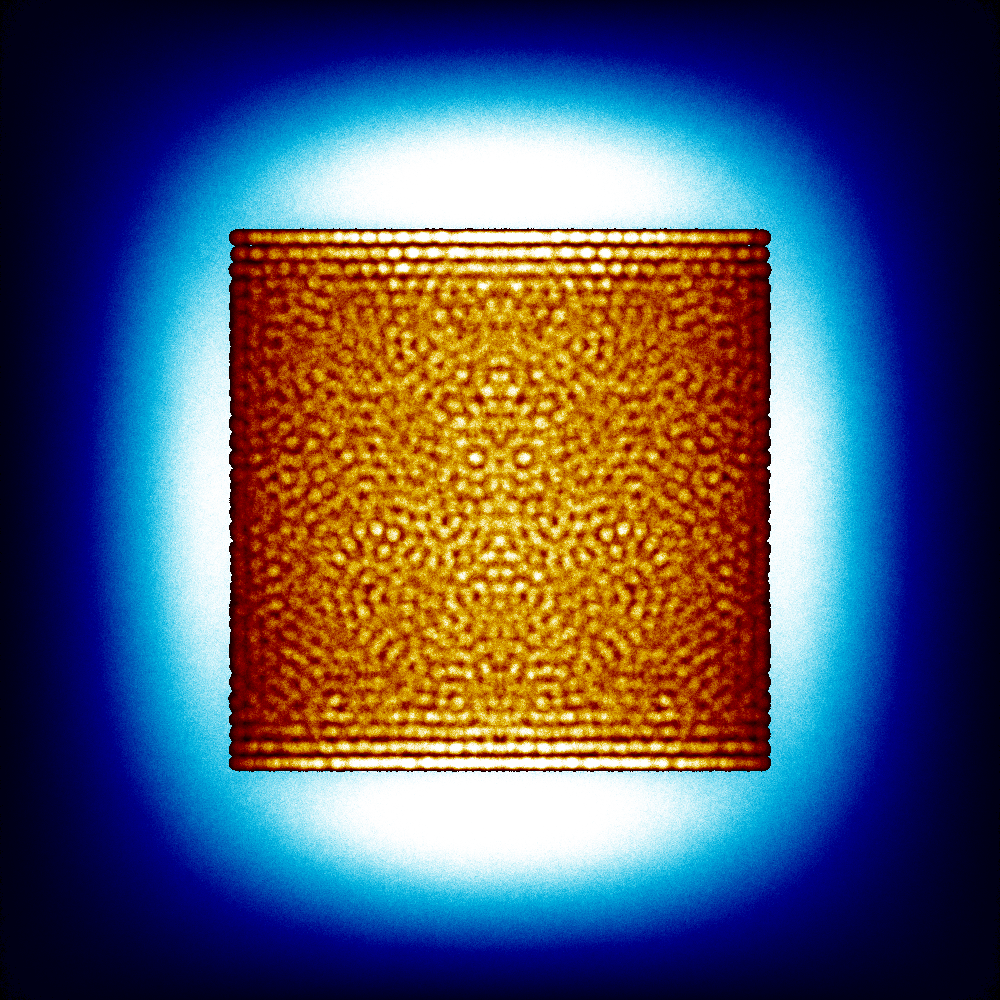
\includegraphics[width=0.95\linewidth]{figures/240-300/240-300-vm}
  \caption{Axial Mesh}
  \label{fig:bstep1}
\end{subfigure}
%
\caption{Sensitivity Analysis: $240^{\circ}$ - $300^{\circ}$}
\label{fig:240-300}
\end{figure}
\begin{itemize}
\item as above, but the 240-300 degree slice
\end{itemize}

\begin{figure}[H]
\centering

\begin{subfigure}{0.45\textwidth}
  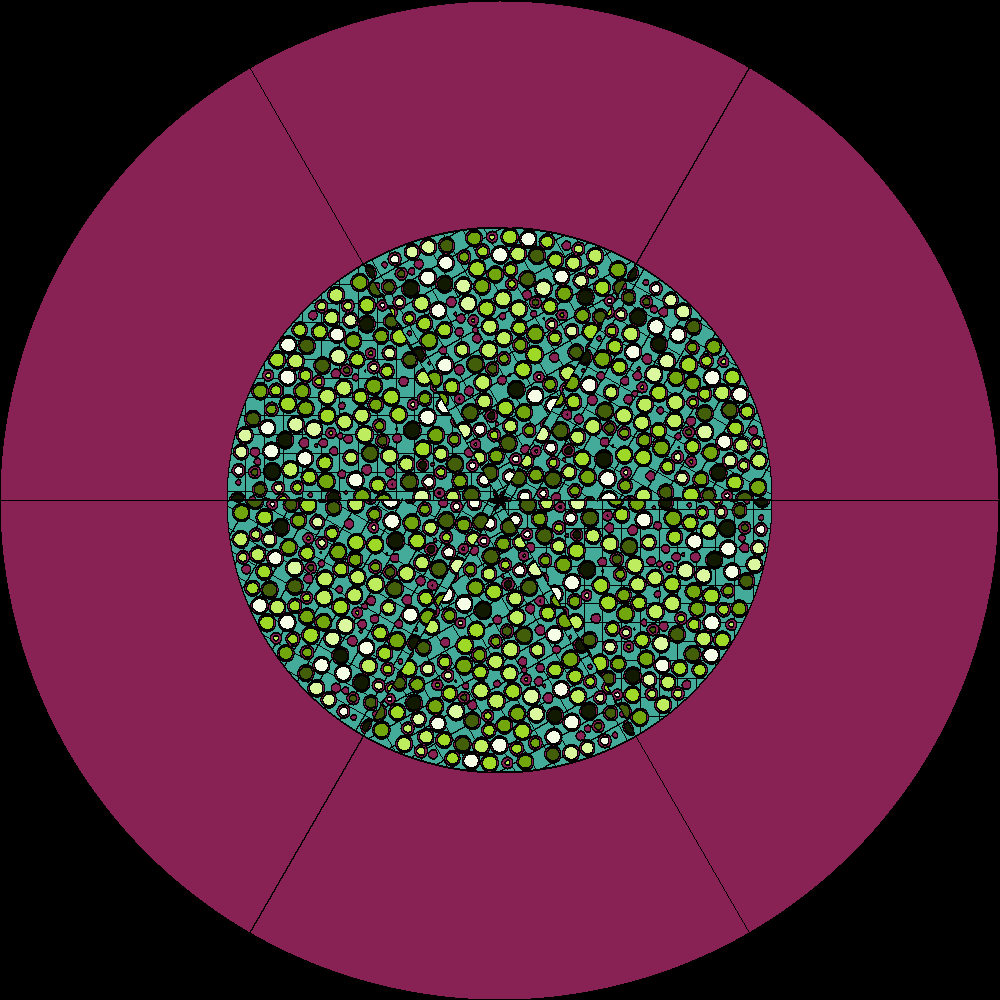
\includegraphics[width=0.95\linewidth]{figures/300-360/300-360-r}
  \caption{Radial Cross Section at y=0}
  \label{fig:bstep0}
\end{subfigure}%
%
\begin{subfigure}{0.45\textwidth}
  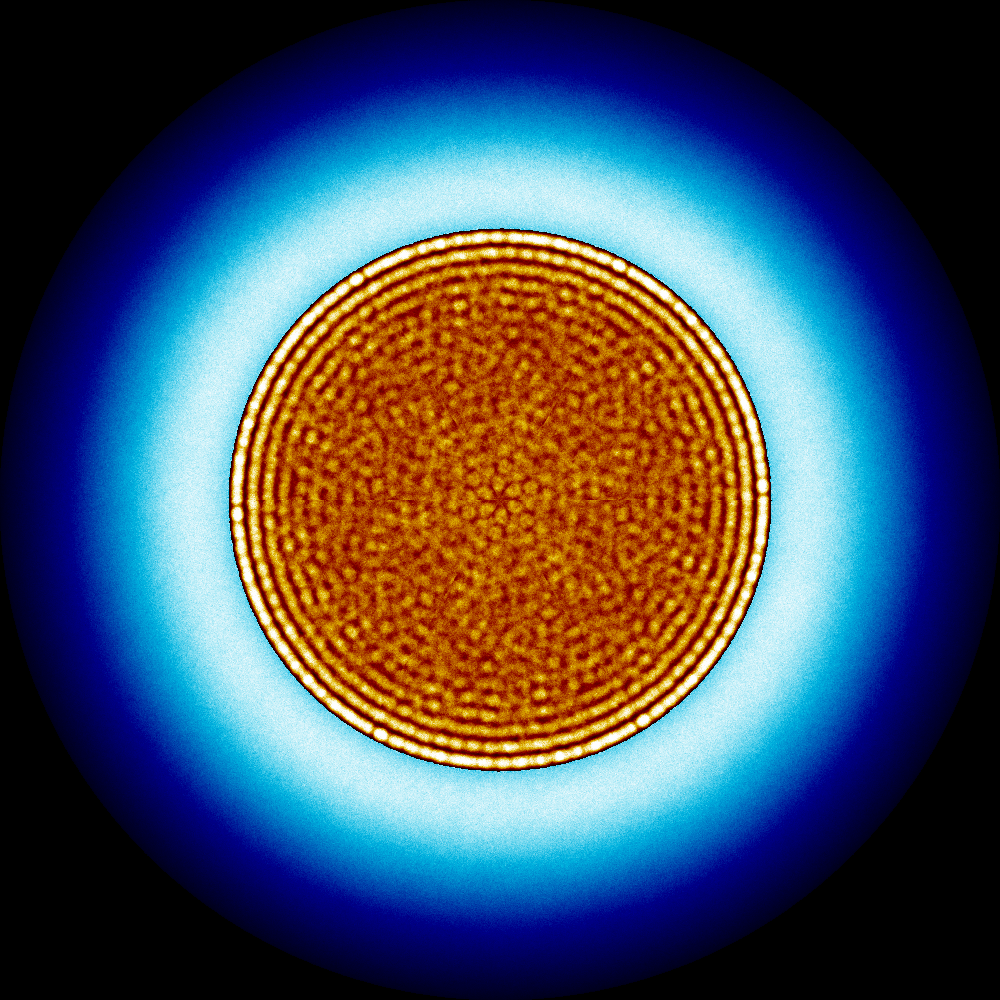
\includegraphics[width=0.95\linewidth]{figures/300-360/300-360-rm}
  \caption{Radial Mesh}
  \label{fig:bstep1}
\end{subfigure}

\begin{subfigure}{0.45\textwidth}
  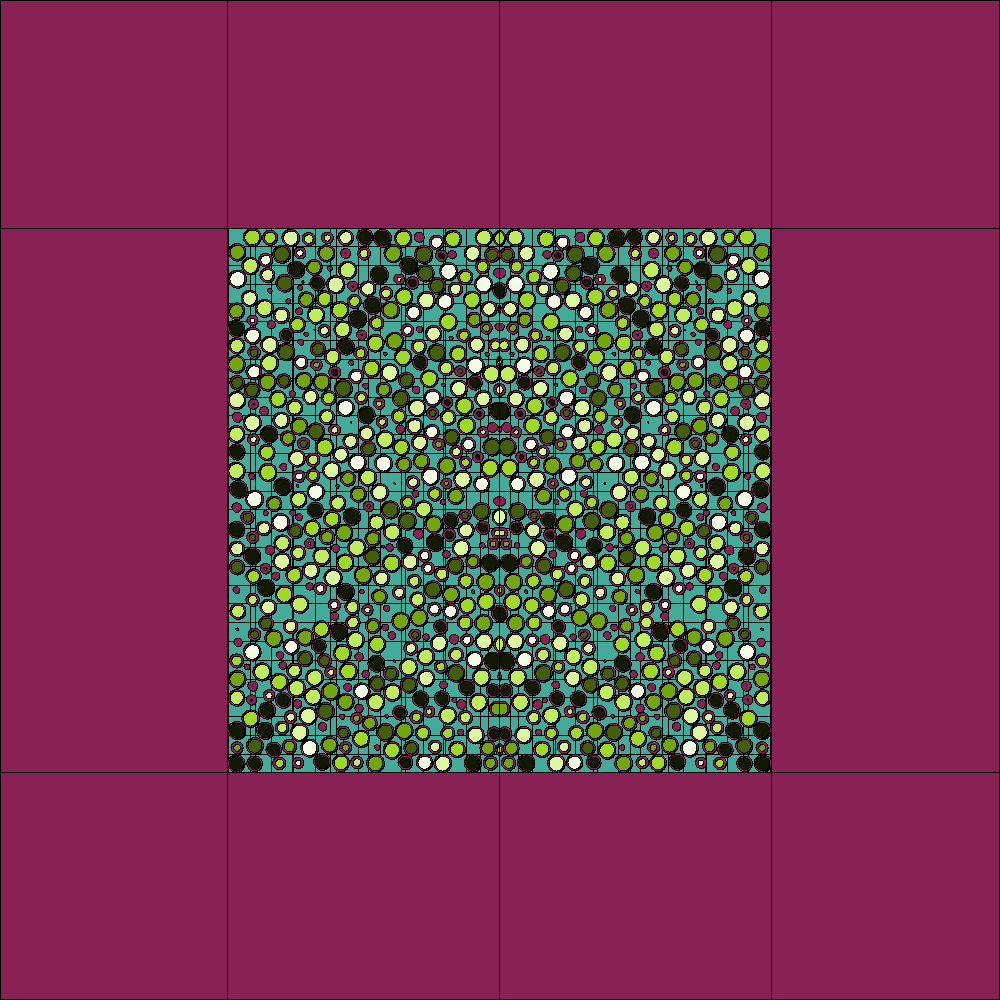
\includegraphics[width=0.95\linewidth]{figures/300-360/300-360-v}
  \caption{Axial Cross Section at z=0 }
  \label{fig:bstep1}
\end{subfigure}
%
\begin{subfigure}{0.45\textwidth}
  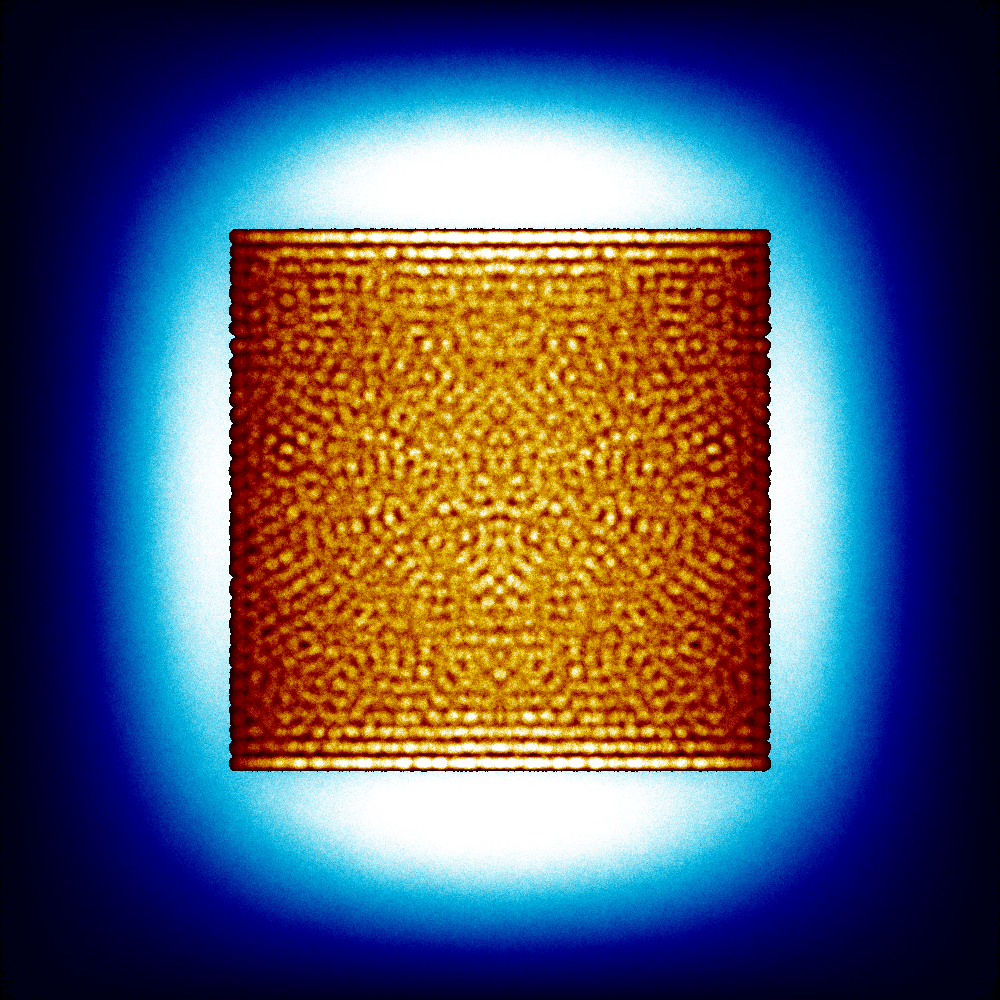
\includegraphics[width=0.95\linewidth]{figures/300-360/300-360-vm}
  \caption{Axial Mesh}
  \label{fig:bstep1}
\end{subfigure}
%
\caption{Sensitivity Analysis: $300^{\circ}$ - $360^{\circ}$}
\label{fig:300-360}
\end{figure}
\begin{itemize}
\item as above, but the 300-360 degree slice
\end{itemize}

\subsection{Effects of Fuel Composition Shuffling}